\chapter{Implementation}

\section{Preparing datasets}

\subsection{Stock Datasets}

There are many stock datasets in literature used to study image recognition techniques, like
\textbf{``Oxford 102 Flowers Dataset''}\autocite{nilsback2008automated},
\textbf{``The Caltech-UCSD Birds-200-2011 Dataset''}\autocite{WahCUB_200_2011}
and \textbf{``The Oxford-IIIT Pet Dataset''}\autocite{parkhi12a} which have 37 species of cats and dogs.
For short, those datasets are called flowers-102, birds-200, and pets-35 respectively.

For toy problems, a much simpler datasets with smaller number of classes are needed.
That's why such datasets were crafted by manipulating previously mentioned datasets.
For example, two classes dataset of ``Cats and Dogs'' was created by adapting pets-37 dataset, merging 12 cats breeds into a ``Cats'' class, and the rest are merged into ``Dogs'' class.
A dataset with three classes ``Cat, Dog or Bird''
was created by merging all pictures from birds-200 dataset into one class
(taking random 3,000 pictures out of around 11,000 pictures),
then add them to the previous ``Cats and Dogs'' dataset.

Another toy dataset is \href{http://download.tensorflow.org/example_images/flower_photos.tgz}{the five flowers dataset}(flowers-5)
containing labeled images for Daisy, Dandelion, Roses, Sunflowers, and Tulips.

\subsection{Vehicle Viewing Angles Dataset}

For the sake of cleaning car images, a small hand-picked dataset was created to identify vehicle viewing angles into nine classes, 

\begin{description}
\item [interior dashboard view], having either steering wheel or odometer visible.
\item [interior seats view] no steering wheel visible nor odometer visible.
\item [front view] both head lights are visible, no doors are visible.
\item [back view] both tail lights are visible, no doors are visible.
\item [side view] both front door and back door visible, both side wheels are visible,
at most one head light visible and at most one tail light visible (if half of radiator grille is visible, then it's front-side view)
\item [front-side view] both front door and back door visible, both side wheels are visible, and both front head lights are visible (or more than half of the radiator grille)
\item [back-side view] both front door and back door visible, both side wheels are visible, and both back tail lights are visible
\item [Wheels] pictures of cars with only one wheel is visible and no-car wheels and alloy wheel.
\item [under-hood]  without headlights or grill visible
\end{description}

Another dataset is created by subdividing each of ``Side view'', ``Back view'', and ``Back-side view'' into six classes:
Sedan, Coupe, Station, Hatchback, SUV, and Pickup or truck.

Those two datasets are hand-picked from various websites, google image search, wikipedia,
and \href{http://opensooq.com}{OpenSooq.com}, to have about 200 image from each class.
Making sure to have different backgrounds, various brands, various models, designs of modern and legacy vehicles
both stock ``staged'' images and natural images.

\subsection{Noisy Vehicle Make-Model-Year Dataset}

\href{http://opensooq.com}{OpenSooq.com} is the leading market place in the middle-east,
having thousands of vehicles for sale added by their owners every day.
Owners upload many pictures of their cars and tag them with make/model/year
among other details (like mileage, transmission, ...etc.).
Opensooq have tons of labeled images. But those user-generated images are noisy,
as they have pictures of registration papers, insurance papers,
inspection papers (local or CarFax), maintenance history, picture of business cards, dealer logos, ..etc.
Beside non-car pictures, sellers upload pictures showing some selling points
like moon roof, leather seats, door lock pin, large wheels size, alloy wheels, under the hood customization.
Those picture (as in figure \ref{fig:noisy}) have no association with any of the desired labels.
Such pictures are important to the seller, but from the point of having pictures that conclude tags like car make and model
those pictures are merely noise.

\begin{figure}[!h]
\centering
\includegraphics[width=\textwidth]{noisy}
\caption{Examples of inconclusive pictures uploaded by sellers}\label{fig:noisy}
\end{figure}

\href{http://opensooq.com}{OpenSooq.com} have generously provided us with hundreds of thousands of pictures of each class.

\begin{itemize}
\item 76 distinct car make
\item more than 1600 classes of make-model
\item more than 20 thousand class of make-model-year
\end{itemize}

Many of 20 thousand classes are distinct only on paper, many of them look similar and should be grouped together
For example, Volkswagen Golf Mk3 looked the same from 1991 to 2002, and Beetle looked almost the same since 1956
as seen in figure \ref{fig:beetle}.
This means that this dataset need a lot of cleanup that is discussed later.

A cleaned dataset was produced based on this dataset, that is discussed in later sections.

\begin{figure}[!htbp]
\centering
    \begin{subfigure}[t]{0.48\textwidth}
        \centering
        \includegraphics[width=\textwidth]{beetle-1956}
        \caption{Original look of Volkswagen Beetle in 1956}
    \end{subfigure}
    \begin{subfigure}[t]{0.48\textwidth}
        \centering
        \includegraphics[width=\textwidth]{beetle-2003}
        \caption{A Type 1 VW Beetle produced in 2003 Puebla, Mexico known as ``Última Edición''}
    \end{subfigure}
    \begin{subfigure}[b]{\textwidth}
        \centering
        \includegraphics[width=\textwidth]{beetle-new-1998}
        \caption{The look of VW new beetle in 1998}
    \end{subfigure}
\caption{Different models of VM beetle}\label{fig:beetle}
\end{figure}

\subsection{Pre-processing Images}

while most CNNs take input of size \(224\times224\),
most datasets have images of varying sizes,
mostly too large images (full HD images or better) as they were scraped from social media or quality websites.
It would be a waste of resources to store and photos of such large sizes.

To unify sizes and make it more suitable to such CNNs,
All images have been re-sized keeping aspect ratio so that it would be at most \(300\times300\)
using the following command from \href{https://www.imagemagick.org/}{ImageMagick Suite}

\begin{verbatim}
$ convert input.jpg -resize 300x300'>' output.jpg
\end{verbatim}

% find opensooq_photos/ -type d | while read a; do mkdir -p "2$a" 2>/dev/null ; done
% find opensooq_photos/ -type f | while read a; do convert "$a" -resize 400x400'>' "2${a/.png/.jpg}" ; done

This is one time job that done once beside different run-time pre-processing done by different CNNs.

\section{Tools}

\begin{itemize}
\item SciKit Learn
\item TensorFlow
\item TensorFlow slim models
\end{itemize}

\section{Procedures}

\subsection{Failure of reduction via pre-processing before CNN}

One of the initial ideas was the use of some pre-processing techniques to 
make input images into sparse ``points of interest'' or ``key points''.
By focusing on smaller number of points,
hoping to get a simpler problem that would require less resources.
Hand crafted ``hit-or-miss'' convolution filters was used
(hits are ones over their count, and misses are minus ones over their count).
One of them those filters was corner filter (in figure \ref{fig:hmt-corner}) which should be applied
in its four variations (rotated 90° each).
Another tried was done using a small empty circle ``hit-or-miss'' (shown in figure \ref{fig:hmt-circle}).
Those were applied to input images then taking local peaks (using ``skimage.feature.peak\_local\_max()'').
The results were comparable to Harris corner filter.

The idea was to make input images sparse to reduce the problem before feeding input images to ANN
hoping to get a simpler problem that would require smaller resources to train.
But ANN takes fixed-sized input or sequences in case on RNN.
That's why the searcher could not make any use of the reduction and
moved to reusing off-the-shelf pre-trained CNN.

\begin{figure}[!htbp]
\centering
    \begin{subfigure}[t]{0.32\textwidth}
        \centering
\[
\frac{1}{3} \cdot
\begin{bmatrix}
0 & +1 & 0 \\
-1 & +1 & +1 \\
-1 & -1 & 0 
\end{bmatrix}
\]
    \end{subfigure}
    \begin{subfigure}[b]{0.65\textwidth}
        \centering
        \includegraphics[width=\textwidth]{hmt-4-corners}
    \end{subfigure}
\caption{Corner hit-or-miss transform convolutional matrix on left, results in blue compared to Harris corner in red}\label{fig:hmt-corner}
\end{figure}

\begin{figure}[!htbp]
\centering
    \begin{subfigure}[b]{0.32\textwidth}
        \centering
\[
\begin{bmatrix}
-\frac{1}{4} & \frac{1}{12} & \frac{1}{12} & \frac{1}{12} & -\frac{1}{4} \\
\frac{1}{12} & 0 & 0 & 0 & \frac{1}{12} \\
\frac{1}{12} & 0 & 0 & 0 & \frac{1}{12} \\
\frac{1}{12} & 0 & 0 & 0 & \frac{1}{12} \\
-\frac{1}{4} & \frac{1}{12} & \frac{1}{12} & \frac{1}{12} & -\frac{1}{4}
\end{bmatrix}
\]
    \end{subfigure}
    \begin{subfigure}[b]{0.65\textwidth}
        \centering
        \includegraphics[width=\textwidth]{hmt-small-circle}
    \end{subfigure}
\caption{Small circle hit-or-miss transform convolutional matrix on left, results in blue}\label{fig:hmt-circle}
\end{figure}

\subsection{Category Adaptation}

Category Adaptation works by finding mapping between 
any of state-of-the-art pre-trained off-the-shelf models
(like \href{http://www.image-net.org/challenges/LSVRC/2012/}{ILSVRC-2012-CLS} winners).
For e-commerce like \href{http://opensooq.com}{OpenSooq.com} 
instead of training a model to identify cars, electronics, ...etc.
one can just map the one thousand ImageNet classes into his/her own classes as in table \ref{table:mapping_os_imagenet},
and flag non-mapped images for human moderation.

Human effort needed to carefully map the one thousand class to relevant categories
is much less than preparing a clear dataset suitable for training.

Passing noisy labeled dataset and taking top most classes (using percentiles) is important in both validating human mappings
and in finding unusual flaws in ImageNet,
for example, images of car inspection papers usually get detected as ``restaurant menu'' or ``website''
and pictures showing car seats might get identified as ``barber chair'' or ``stretcher''.

The benefit of ``Category Adaptation'' that it does not require training nor preparing dataset.
On the other hand, it can't get fine-grained, as you can merge categories but you can't divide them,
for example you can not identify different vehicle types (Sedan, Hatchback, SUV, ...etc.), makers, models.
You can't add new categories, for example smart phones might be detected as modems or other older devices that
were part of \href{http://www.image-net.org/challenges/LSVRC/2012/}{ILSVRC-2012-CLS} database\autocite{deng2012imagenet}.

\begin{table*}\caption{Example of ``Category Adaptation'' hand-picked mapping of ImageNet classes to some of OpenSooq e-Commerce Categories}\label{table:mapping_os_imagenet}
\begin{tabularx}{\textwidth}{lX}
\toprule
OpenSooq Label & ImageNet Label \\
\midrule
\multirow{14}{*}{Autos} & beach wagon \\
 & minivan \\
 & jeep \\
 & limousine \\
 & convertible \\
 & pickup \\
 & minibus \\
 & sports car \\
 & tow truck \\
 & ambulance \\
 & cab \\
 & racer \\
\midrule
\multirow{12}{*}{Electronics} & cellular telephone, cellphone, mobile phone \\
 & desktop computer \\
 & dishwasher, dish washer, dishwashing machine \\
 & joystick \\
 & laptop, laptop computer \\
 & modem \\
 & printer \\
 & refrigerator, icebox \\
 & remote control, remote \\
 & television, television system \\
 & vacuum, vacuum cleaner \\
 & washer, automatic washer, washing machine \\
\bottomrule
\end{tabularx}
\end{table*}

\subsection{Understanding Weights}

In case of usual ANN, the last layer (the fully connected layer) takes features and multiply them with weights matrix
(\(n\times m\) matrix where \(n\) is number of input features, and \(m\) is number of classes),
add bias and then apply the activation function, then apply ``softmax()'' to convert them to probability like results.
Some CNN have that usual ANN fully connected layer as last layer while others have an equivalent \(1\times1\) convolution
of depth \(m\). In both cases we can have a weights matrix of size \(n\times m\).
As in equation \ref{eq:ann_weights} we can look
to the weights matrix as if it's composed of \(m\) vectors \(\vec{v}_i\) in feature space of dimension \(n\).
Each vector \(\hat{v}_i\) represent the direction of that class, and
the magnitude of the vector is used to control the probability when two classes are activated by same features.

\begin{equation}
W_{n\times m} =
\begin{bmatrix}
w_{11} & w_{12} & \cdots  &  w_{1m} \\
w_{21} & w_{22} & \cdots  &  w_{2m} \\
\vdots  & \vdots  & \ddots  &  \vdots  \\
w_{n1} & w_{n2} & \cdots  &  w_{nm}
\end{bmatrix}
=
\begin{bmatrix}
\vec{v}_{1} & \vec{v}_{2} & \cdots & \vec{v}_{m}
\end{bmatrix}
\label{eq:ann_weights}
\end{equation}

\subsection{Using Category Adaptation to Cleanup Dataset}

As mentioned before \href{http://opensooq.com}{OpenSooq.com} provided the researcher with
a ``Noisy Vehicle Make-Model-Year Dataset''.
``Category Adaptation'' was used to clean this dataset by removing non-cars pictures from it.

A tool named ``img-grep'' that is inspired by UNIX philosophy
and \href{http://pubs.opengroup.org/onlinepubs/009695399/utilities/grep.html}{UNIX grep utility} was created .
This tool reads image file names from standard input,
and output only matching file names (or non-matching if --exclude is passed).
The matching criteria is either a list of label indices or a file containing such label indices. 

Using mapping as in table \ref{table:mapping_os_imagenet}, non-car images were removed from dataset,
surprisingly more 20\% of images were removed, which is understandable because on average a car post have 5 images
one of them is a picture of some papers (registration/inspection).

\begin{program}
\begin{verbatim}
#! /bin/bash
find src -type f -name '*.jpg' | \
  img-grep --model_dir inception_v1 \
    --idx 437,657,610,628,512,718,655,818,865,408,469,752 |
  while read filename
  do
    cp "${filename}" "${filename/src/dst}"
  done
\end{verbatim}
\caption{A simple bash script that uses ``img-grep'' to create a cleaned up version of dataset}
\end{program}


\subsection{Category Adaptation using weights manipulations}

One can produce cars vs. electronics using category adaptation
by mapping classes of the results as in table \ref{table:mapping_os_imagenet}.
One might consider doing this by simply averaging vectors of source classes to be merged in one target class

\begin{equation}
\vec{v}_{t} = ( \vec{v}_1+\vec{v}_2+\ldots+\vec{v}_k ) / k
\label{eq:cat_adapt_avg}
\end{equation}

or even better using unit vectors adjusted by its probability in target task \(p_i\)
and the result vector magnitude is set to be the average magnitude in source task
if we are constructing a target model from scratch or the average magnitude in acceptor model
in case of knowledge transfer to an existing target model.

\begin{equation}
\vec{v'}_{t} = \frac{ \sum\nolimits_{i} p_{i}\hat{v}_i }{ \sum\nolimits_{i} p_{i} }
\label{eq:vec_cat_adapt}
\end{equation}
\begin{equation}
\vec{v}_{t} = \bar{V} \hat{v'}_{t}
\label{eq:vec_cat_adapt2}
\end{equation}


\subsection{Application on ``Cats, Dogs and Birds'' dataset}

As discussed before\ref{eq:ann_weights} the weights matrix is composed of vectors in feature space,
one can use a formula to \ref{eq:vec_cat_adapt} create weights.
A small number of pictures were passed from ``Cats, Dogs, and Birds'' dataset,
exactly 100 pictures (out of thousands) from each of the three classes to Inception v1 pre-trained on ImageNet
to find probability of donor class in target class and got results as in table \ref{table:inception_cats}.

\begin{table*}\caption{Results of passing some cats, dogs and birds pictures to ImageNet Inception v1}\label{table:inception_cats}
\begin{adjustwidth}{-2in}{-2in} %
\centering
\begin{tabular}{@{}lrl@{}}
\toprule
Target Class & Probability \(p_i\) & Donor Model Class \\
\midrule
\multirow{3}{*}{Cat} & 49\% & 286:Egyptian cat \\
 & 19\% & 285:Siamese cat \\
 & 10\% & 284:Persian cat \\
 & 10\% & 282:tabby cat \\
 & 2\% & 288:lynx, catamount \\
\midrule
\multirow{9}{*}{Dog} & 14\% & 181:pit bull terrier \\
 & 10\% & 243:boxer \\
 & 8\% & 213:English setter \\
 & 5\% & 211:German short-haired pointer \\
 & 5\% & 200:Scotch terrier \\
 & 4\% & 262:keeshond \\
 & 4\% & 259:Samoyed \\
 & 4\% & 256:Leonberg \\
 & 3\% & 258:Great Pyrenees \\
 & 3\% & 248:Saint Bernard \\
 & 3\% & 238:miniature pinscher \\
 & 3\% & 203:soft-coated wheaten terrier \\
 & 3\% & 188:Yorkshire terrier \\
 & 3\% & 163:beagle \\
 & 2\% & 274:Canis dingo \\
 & 2\% & 264:Pembroke \\
 & 2\% & 257:Newfoundland dog \\
 & 2\% & 220:cocker spaniel \\
 & 2\% & 158:papillon \\
 & 2\% & 154:Maltese dog \\
\midrule
\multirow{9}{*}{Bird} & 10\% & 11:brambling \\
 & 9\% & 17:bulbul \\
 & 9\% & 13:linnet \\
 & 6\% & 147:albatross, mollymawk \\
 & 6\% & 12:goldfinch, Carduelis carduelis \\
 & 5\% & 20:chickadee \\
 & 5\% & 19:magpie \\
 & 5\% & 18:jay \\
 & 4\% & 96:jacamar \\
 & 4\% & 144:oystercatcher \\
 & 4\% & 14:snowbird \\
 & 3\% & 95:hummingbird \\
 & 3\% & 22:kite \\
 & 3\% & 16:Turdus migratorius \\
 & 2\% & 93:bee eater \\
 & 2\% & 92:coucal \\
 & 2\% & 21:water ouzel \\
 & 2\% & 15:indigo bird \\
 & 2\% & 134:bittern \\
 & 2\% & 129:black stork \\
\bottomrule
\end{tabular}
\end{adjustwidth}


\end{table*}

\subsection{Fine Tuning off-the-shelf models}

Fine-Tuning an already trained model work by reconstructing a new ANN,
transferring weights from the pre-trained network (called donor model or source model)
to the newly constructed one (called acceptor or target model)
up to some point as seen in figure \ref{fig:ann4}.

Weights transferred from the donor model carries already learned knowledge on how to extract features and
how to pre-process them\autocite{oquab2014learning}.
On the other hand, weights left to be trained are the decision making parts (decision making layer),
which is not transferred but left to be trained on target task which might be different than source task.

The same thing with ConvNets as seen in figure \ref{fig:cnn-doner-acceptor},
as they typically have some fully connected layers (just like usual ANN) toward the end,
or have an equivalent 1x1 convolution that act as a fully connected ANN layer,
that leads to the classes after being passed to softmax function.

Fine-tuning an existing model gives state-of-art accuracy\autocite{ouyang2016factors}
with fraction of training time (compared to fully train the new model)
as millions of weights are transferred from the donor model without training.


If training one layer was not enough to get the desired accuracy,
one might add more fully connected layers toward the end of the network
or include more layers in the trainable parts (blue colored layers in figure \ref{fig:ann4}).

\begin{figure}[!h]
\centering
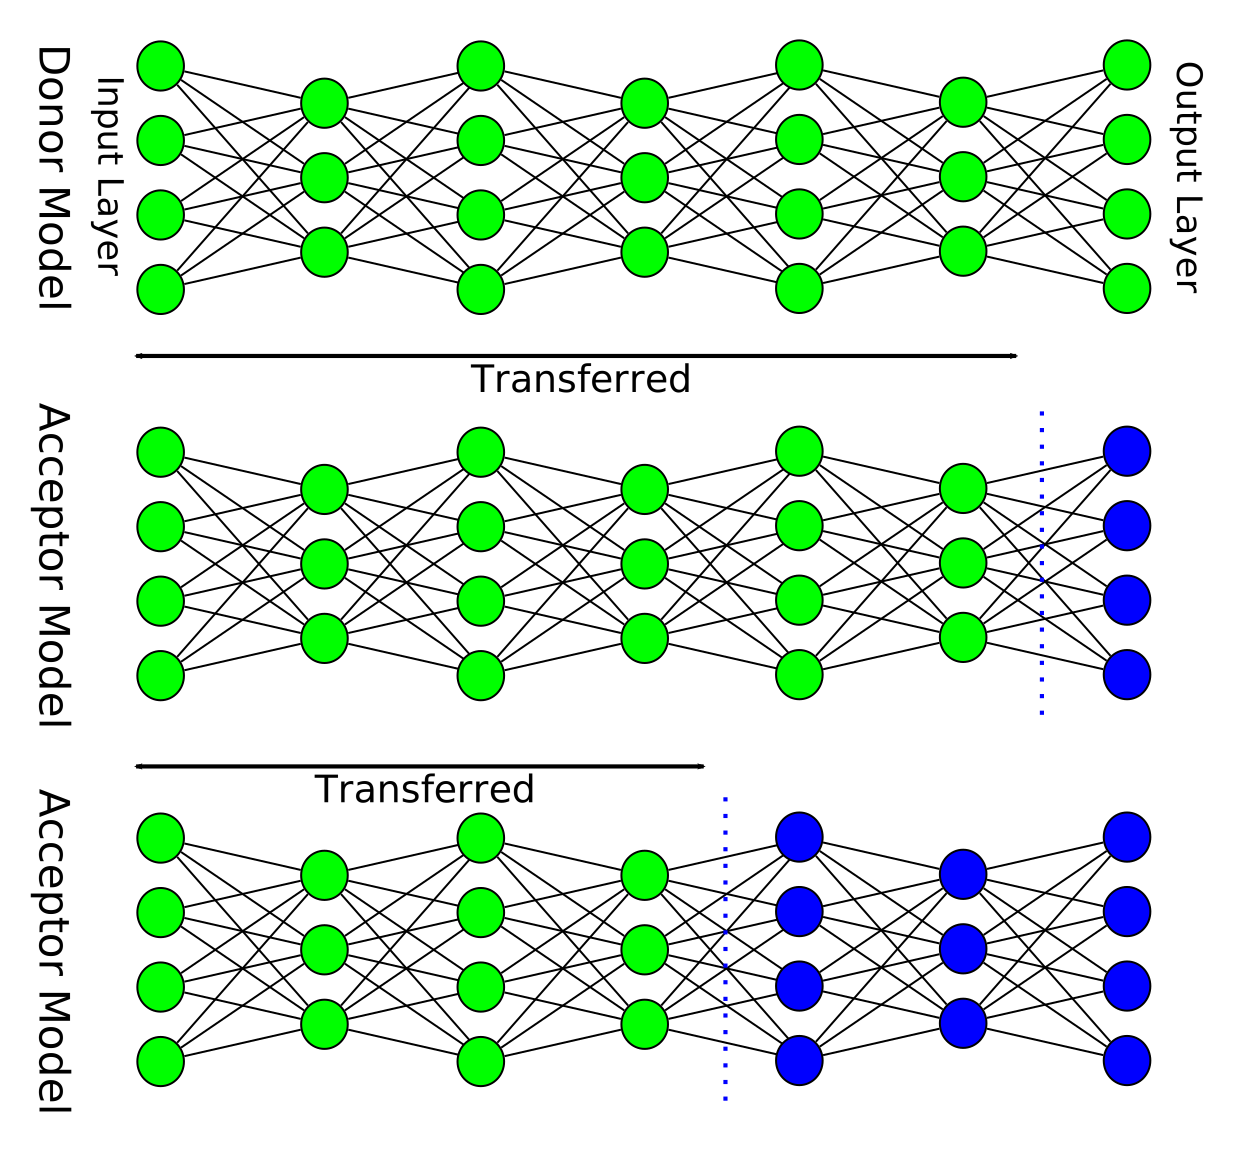
\includegraphics[width=0.7\textwidth]{ann4}
\caption{How weights are transfered from the donor model to the acceptor model in ANN}\label{fig:ann4}
\end{figure}


\begin{figure}[!h]
\centering
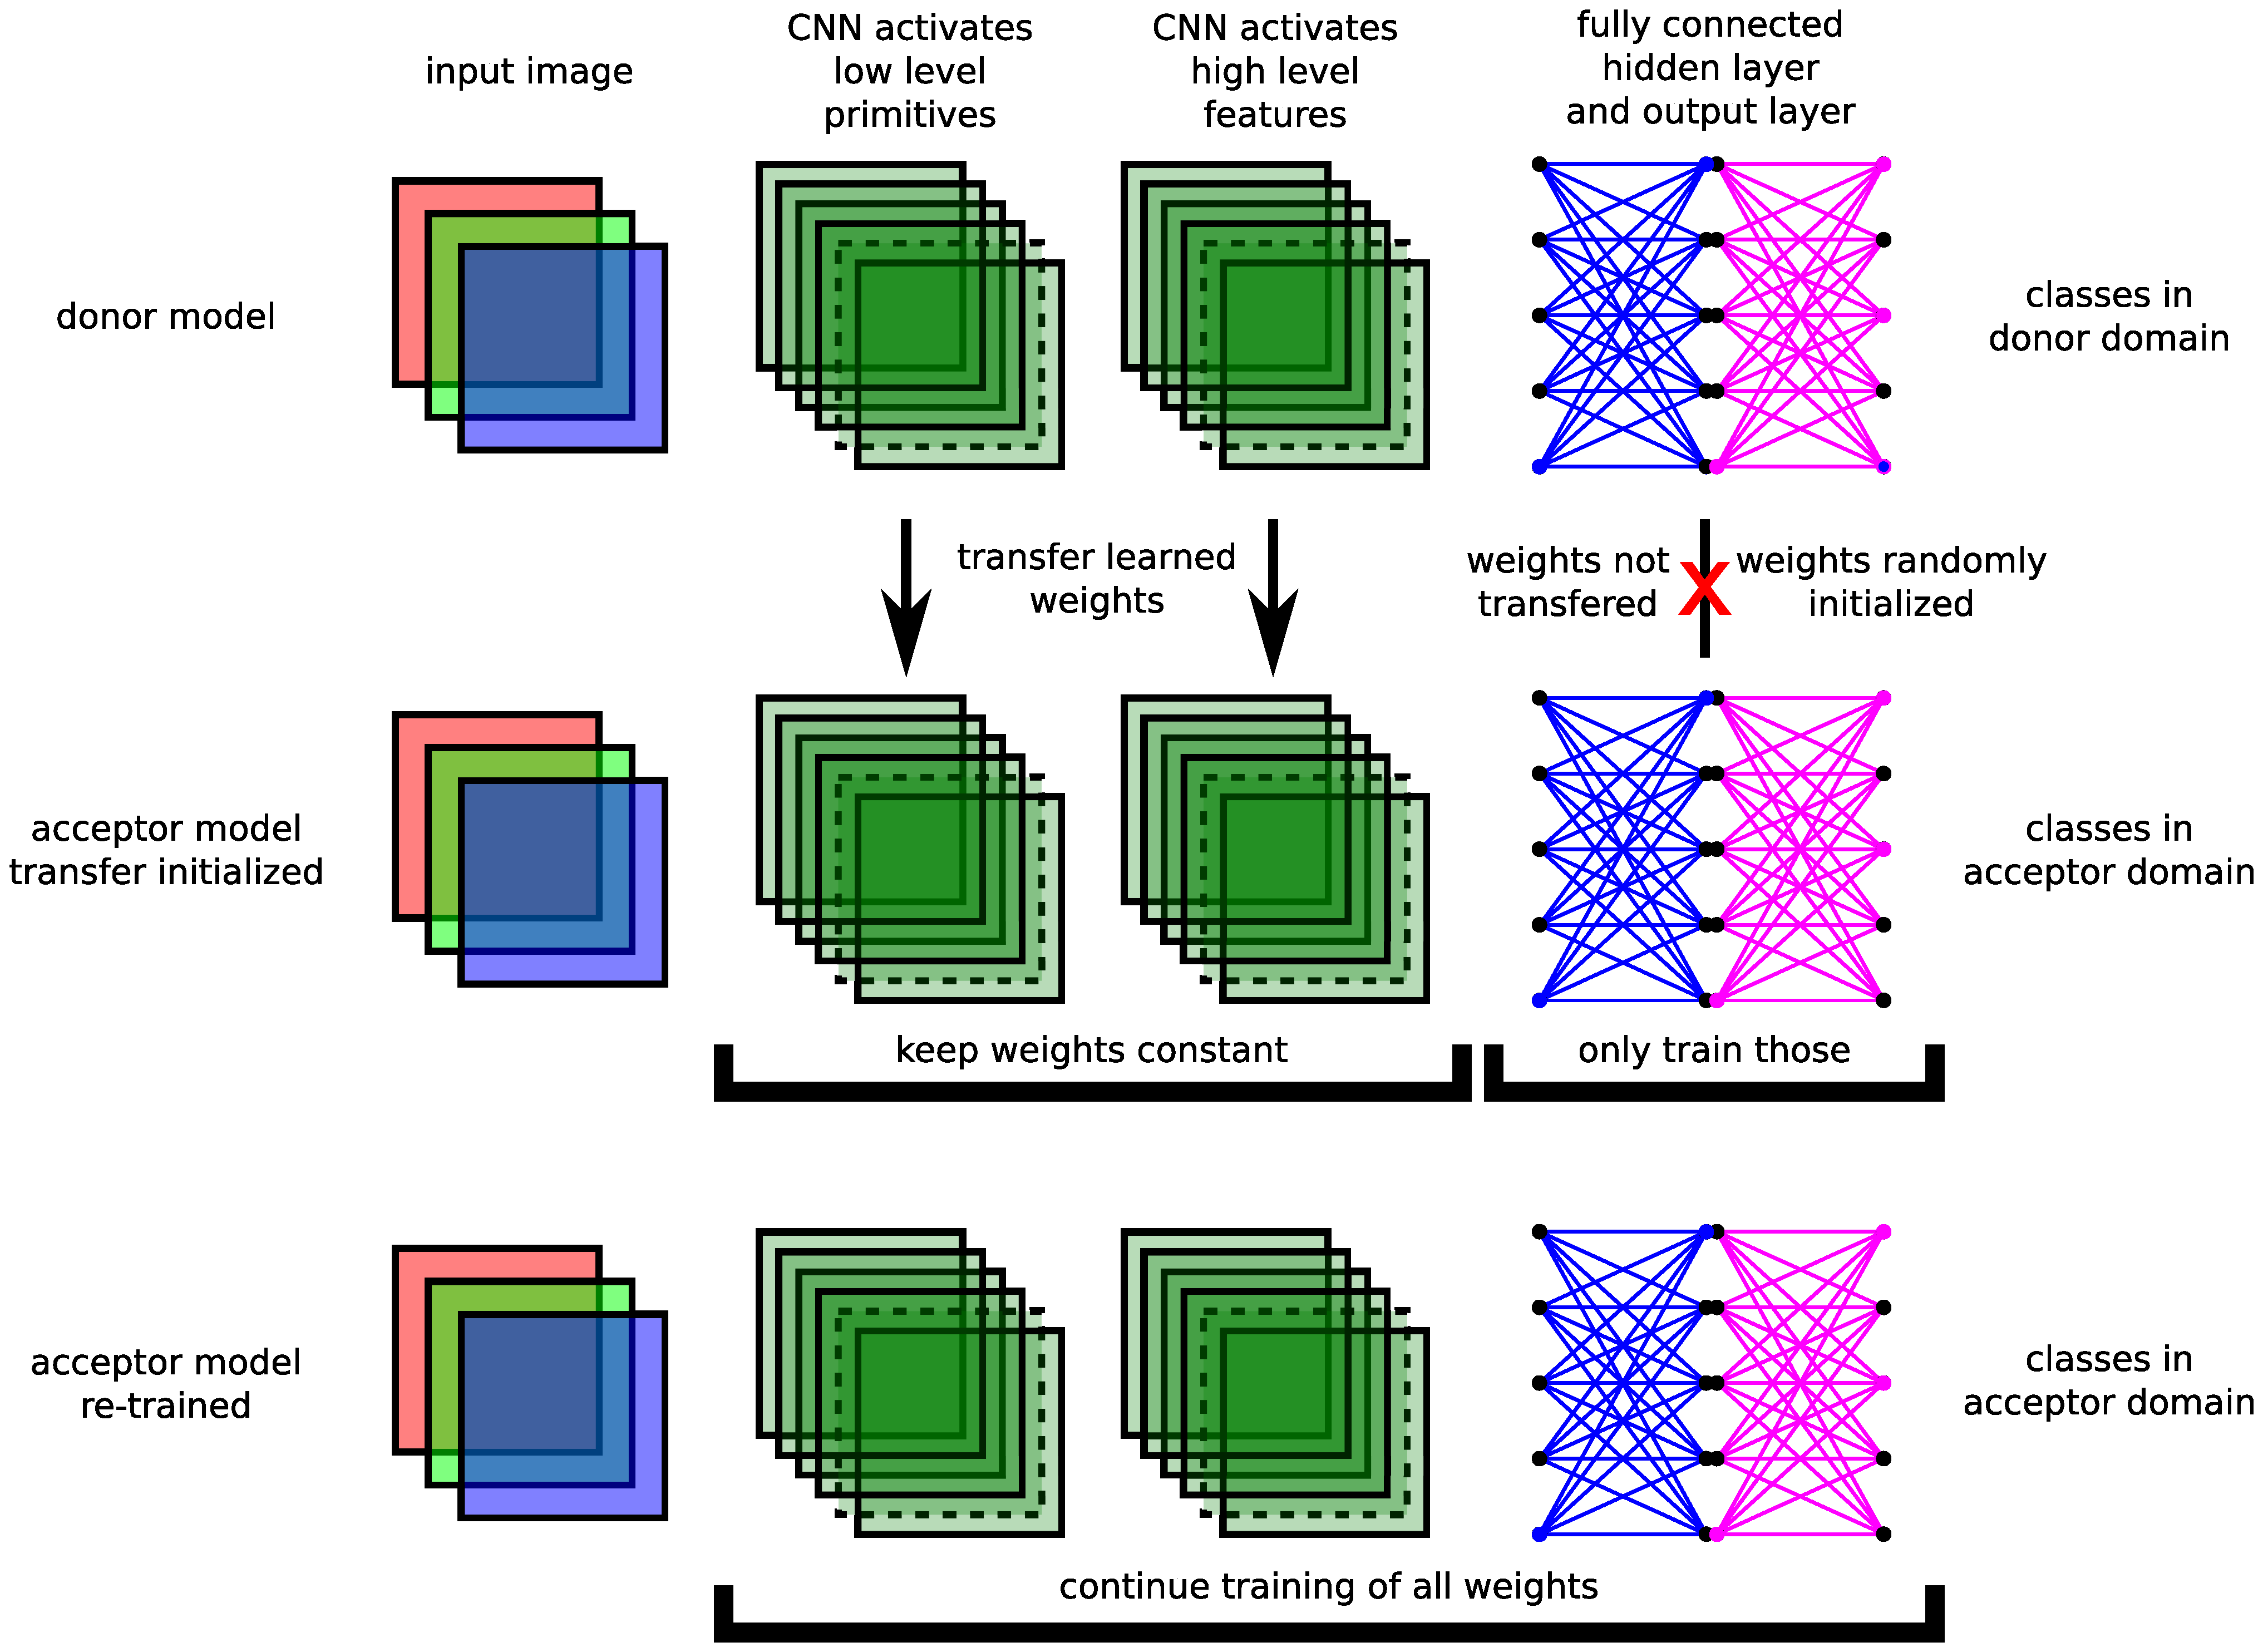
\includegraphics[width=0.7\textwidth]{cnn-doner-acceptor}
\caption{How weights are transfered from the donor model to the acceptor model in CNN}\label{fig:cnn-doner-acceptor}
\end{figure}

\subsection{Estimating performance of fine-tuning off-the-shelf models}


Fine-tuning some models were found to be way more slower than others,
to identify the factors that affects the speed of training and fine-tuning,
two networks that have very different properties were studied:
VGG-16\autocite{simonyan2014very} which has 15 billion multiplication-accumulation operations and around 140 million weights
75\% of which are in a single bottleneck layer (that is FC6), 
and GoogLeNet or Inception v1\autocite{szegedy2015going} which have small fraction of that, that is
less than 1.5 billion multiplication-accumulation operations and less than ten million weights
and the weights are almost evenly distributed on layers.

The number of weights left for training varies from model to another,
so do number of multiplication-accumulation operations, for example,
assuming you have \(n\) classes, in VGG-16\autocite{simonyan2014very},
the fully connected layers are FC6, FC7, and FC8,
one can just retrain FC8 (which has \(4096\times n\) weights)
or the whole fully connected ANN starting from FC6 (which is 120 million more weights than FC8 only).
or the whole CNN network having 138 million weights,
for more details refer to table \ref{table:vgg}.

All experiments in this section were done with 8 images per batch per step, and measure the time needed to reach 500 steps.
Table \ref{table:fine-tune-vgg16} shows the time and accuracy of different fine-tuning settings
of VGG16\autocite{simonyan2014very} on toy dataset of \href{http://download.tensorflow.org/example_images/flower_photos.tgz}{five flowers}

VGG16\autocite{simonyan2014very} pre-trained on ImageNet's ILSVRC 2012\autocite{deng2012imagenet}
which was previously analyzed in table \ref{table:vgg}.
The number of multiplication/addition operations is about 15,470M operation
to be exact it's \(15466168320+4096\times n\) where \(n\) is number of classes.
The number of weights to be trained is last layer (named ``FC8'') is \( 4096\times n \),
while number of weights in previous layers does not depend on number of classes.
As you can see in that table most weights (74.3\%) are in ``FC6'' layer.

Formula \ref{eq:t1} estimates training time by assuming it's proportional to number of multiplication/addition operations \(M\)
in forward pass and number of trainable weights \(W\)
and number of multiplication/addition operations in training part \(T\)
which is the same as the number of trainable weights times output width and height (which is usually \(1\times 1\).
Needless to say that those constants depends on the speed of the machine, how it's configured,
how it handles parallelism, and the model design itself (like non-weights operations like pooling, pre-processing, ..etc.).

\begin{equation}
t = C_0 + C_1 \cdot M + C_2 \cdot W + C_3 \cdot T
\label{eq:t1}
\end{equation}

To find \(C_0\) (which is the time to load the model and store it without training),
just run zero steps, and that was 8 seconds.
To find \(C_1\), \(C_2\), and \(C_3\), by substituting last 3 rows from table \ref{table:fine-tune-vgg16}
we get the following linear equation.

\begin{equation}
\begin{bmatrix}
15,466,188,800 &  16,797,696 &  16,797,696 \\
15,466,188,800 & 119,558,144 & 119,558,144 \\
15,466,188,800 & 121,917,440 & 581,980,160
\end{bmatrix}
\times x = 
\begin{bmatrix}
  772.9-8 \\
2,012.242-8 \\
2,016.7-8
\end{bmatrix}
\label{eq:t_vgg}
\end{equation}

we get 

\[ C_1 = 3.64 \times 10^{-8} \]
\[ C_2 = 1.21 \times 10^{-5} \]
\[ C_3 = -5.21 \times 10^{-8} \]

Having negative value for \( C_3 \) indicate that assumption should be changed by removing the term \(C_3 \cdot T\)
removing the effect of number of trainable weights as in formula \ref{eq:t2}

\begin{equation}
t = C_0 + C_1 \cdot M + C_2 \cdot W
\label{eq:t2}
\end{equation}

By substituting first and last rows, and solve the linear equation \ref{eq:t_vgg2}

\begin{equation}
\begin{bmatrix}
15,466,188,800 &      20,480 \\
15,466,188,800 & 121,917,440 
\end{bmatrix}
\times x = 
\begin{bmatrix}
 582.8-8 \\
2016.7-8
\end{bmatrix}
\label{eq:t_vgg2}
\end{equation}

We get

\[C_1=3.71\times 10^{-8} \]
\[C_2=1.18\times 10^{-5} = 316.8 \times C_1 \]

Writing \(C_2\) and \(C_3\) in terms of \(C_1\), we got \ref{eq:t3}

\begin{equation}
t = 8 + C_1 \cdot M + 316.8  C_1 \cdot W
\label{eq:t3}
\end{equation}

Using \ref{eq:t3} substituting second and third rows of table \ref{table:fine-tune-vgg16} 

\[ t_{fc7} = 8 + C_1 \times 15,466,188,800 + C_2 \times  16,797,696 =   780.1 \]
\[ t_{fc6} = 8 + C_1 \times 15,466,188,800 + C_2 \times 119,558,144 = 1,988.9 \]

which is very close from actual value of 772.9 and 2,012.2 with error 0.9\% and 1.1\% respectively.

Repeating same experiment with different dataset, this time with Birds 200\autocite{WahCUB_200_2011},
results are shown in table \ref{table:fine-tune-vgg16-birds200}. Using formula \ref{eq:t1} gave very close values

\[ C_1 = 3.62\times 10^{-8} \]
\[ C_2 = 1.23\times 10^{-5} \]
\[ C_3 = -5.44\times 10^{-8} \]

And when omitting \(T\) term as in formula \ref{eq:t2}, we got the following result

\[ C_1 = 3.69\times 10^{-8} \]
\[ C_2 = 1.20\times 10 ^{-5} = 324.4 C_1 \]
\[ t = 8 + C_1 \cdot M + 324.4  C_1 \cdot W \]

which is very close from our previous result.

Although the cost of trainable weights is 353 times that of multiplications,
in case of fine-tuning last layer as in FC8 layer,
number of multiplication-accumulation operations \(M\)
is 755 thousand times greater than number of trainable weights \(W\).

This huge gap between number multiplication-accumulation operations 
and number weights in case of fine-tuning neglect any effect of number of classes on time
The cost is merely controlled by number of multiplication-accumulation operations in forward pass is almost constant 15,466M
as seen in table \ref{table:fine-tune-vgg16-2}.
Same conclusion applies to Inception v1 as seen in table \ref{table:fine-tune-inception-v1}
where the number of classes does not have any effect of time with fixed trainable layers.

Several experiments were applied on fine-tuning different layers of Inception V1
and results were recorded on table \ref{table:fine-tune-inception-v1}.
Forming an equation similar to \ref{eq:t2} by substituting the time of fine-tuning a single layer of Inception V1
on flowers 5 dataset and that of fine-tuning both last layer and last inception block ``Mixed\_5c''

\begin{equation}
\begin{bmatrix}
1,497,357,312 &     5,120 \\
1,497,357,312 & 1,349,632 \\
\end{bmatrix}
\times x = 
\begin{bmatrix}
 94.0-8 \\
102.8-8
\end{bmatrix}
\label{eq:t_inception_v1_1}
\end{equation}

Solving it would result in:

\[ C1 = 5.74\times 10^{-8} \]
\[ t = 8 + C_1 \cdot M + 114.0  C_1 \cdot W \]

and by applying it on fine-tuning last layer and last two inception blocks ``Mixed\_5c'' and ``Mixed\_5b''

\[ t = 8 + C_1 \cdot M + 114.0  C_1 \cdot W \]
\[ t = 8 + 1,497,357,312 c1 + 2,326,528 c2 = 109.2 \]

which matches the actual observed value of \( 109.5 \) seconds with error of \(0.3\) seconds.

When more classes are included, converging becomes slower as it's harder to reach good accuracy
this is seen in tables \ref{table:fine-tune-vgg16-2} and \ref{table:fine-tune-inception-v1}.

The time needed to fine-tune last layer of Inception V1 is \(3.7\times\)
faster than full training (as in table \ref{table:fine-tune-inception-v1})
and with VGG-16 it's \(5.6\times\) faster (as in table \ref{table:fine-tune-vgg16}).

Not only it's faster but also better accuracy, because:

\begin{itemize}
\item it can run more training steps in same amount of time.
\item all convolution filters/pre-processors and high-level feature-extractors are already trained.
\end{itemize}

This is only valid up to a limit, because the second point does not hold,
the target task might require different pre-processing or feature extractor than source task
to achieve the desired accuracy, in that case fine-tuning can be used for initialization.

\begin{table*}\caption{Comparing fine-tuning VGG-16 performance up to different layers on same Flowers-5 dataset}\label{table:fine-tune-vgg16}
\centering
\begin{small}
\begin{tabularx}{\textwidth}{llrrrrrr}
\toprule
Model & Layer & Classes & \makecell{Total \\ Mults} & \makecell{Trainable \\ Weights} & \makecell{Training \\ Mults} & Time & Accuracy \\
\midrule
VGG-16 & FC8     & 5 & 15,466M &      20K &         20K &   582.8s & 80.0\% \\
VGG-16 & FC7     & 5 & 15,466M &  16,798K &     16,798K &   772.9s & 76.1\% \\
VGG-16 & FC6     & 5 & 15,466M & 119,558K &    119,558K & 2,012.2s & 45.9\% \\
VGG-16 & Conv5-3 & 5 & 15,466M & 121,917K &    581,980K & 2,016.7s & 57.6\% \\
\midrule
VGG-16 & All     & 5 & 15,466M & 134,269K & 15,466,189K & 3,249.8s & 42.7\% \\
\bottomrule
\end{tabularx}
\end{small}
\end{table*}

\begin{table*}\caption{Comparing fine-tuning VGG-16 performance up to different layers on Birds-200 datasets\autocite{WahCUB_200_2011} }\label{table:fine-tune-vgg16-birds200}
\centering
\begin{small}
\begin{tabularx}{\textwidth}{llrrrrrr}
\toprule
Model & Layer & Classes & \makecell{Total \\ Mults} & \makecell{Trainable \\ Weights} & \makecell{Training \\ Mults} & Time & Accuracy \\
\midrule
VGG-16 & FC8     & 200 & 15,467M &     819K &     819K &   588.6s & 22.8\% \\
VGG-16 & FC7     & 200 & 15,467M &  17,596K &  17,596K &   784.1s & 10.0\% \\
VGG-16 & FC6     & 200 & 15,467M & 120,357K & 120,357K & 2,043.9s & 00.5\% \\
VGG-16 & Conv5-3 & 200 & 15,467M & 122,716K & 582,779K & 2,047.8s & 00.3\% \\
\bottomrule
\end{tabularx}
\end{small}
\end{table*}

\begin{table*}\caption{Comparing fine-tuning same layer of VGG-16 network on different datasets}\label{table:fine-tune-vgg16-2}
\centering
\begin{small}
\begin{tabularx}{\textwidth}{llrrrrrr}
\toprule
Model & Layer & Dataset & \makecell{Total \\ Mults} & \makecell{Trainable \\ Weights} & \makecell{Training \\ Mults} & Time & Accuracy \\
\midrule
VGG-16 & FC8  & Cats Dogs 2   & 15,466,176,512 &   8,192 &   8,192 &   582.4s & 99.3\% \\
VGG-16 & FC8  & Flowers 5     & 15,466,188,800 &  20,480 &  20,480 &   582.8s & 80.0\% \\
VGG-16 & FC8  & Pets 37       & 15,466,319,872 & 151,552 & 151,552 &   582.6s & 82.9\% \\
VGG-16 & FC8  & Flowers 102   & 15,466,586,112 & 417,792 & 417,792 &   584.0s & 57.8\% \\
VGG-16 & FC8  & Birds 200     & 15,466,987,520 & 819,200 & 819,200 &   588.6s & 22.8\% \\
\bottomrule
\end{tabularx}
\end{small}
\end{table*}

\begin{table*}\caption{Comparing fine-tuning Inception V1 performance up to different layers on different datasets}\label{table:fine-tune-inception-v1}
\centering
\begin{small}
\begin{tabularx}{\textwidth}{llrrrrrr}
\toprule
Model & Layer & Dataset & Total Mults & \makecell{Trainable \\ Weights} & Time & Accuracy \\
\midrule
Inception V1 & Logits   & Cats Dogs 2   & 1,497,354,240 &     2,048 &   94.0s & 99.3\% \\
Inception V1 & Logits   & Flowers 5     & 1,497,357,312 &     5,120 &   94.1s & 71.8\% \\
Inception V1 & Logits   & Pets 37       & 1,497,390,080 &    37,888 &   94.3s & 75.0\% \\
Inception V1 & Logits   & Flowers 102   & 1,497,456,640 &   104,448 &   94.1s & 18.8\% \\
Inception V1 & Logits   & Birds 200     & 1,497,556,992 &   204,800 &   94.6s & 2.2\% \\
\midrule
Inception V1 & Mixed\_5c & Flowers 5     &  1,497,357,312 & 1,349,632 & 102.8s & 75.0\% \\
Inception V1 & Mixed\_5c & Birds 200     &  1,497,556,992 & 1,549,312 & 103.5s & 8.0\% \\
\midrule
Inception V1 & Mixed\_5b & Flowers 5     &  1,497,357,312 & 2,326,528 & 109.5s & 79.2\% \\
Inception V1 & Mixed\_5b & Birds 200     &  1,497,556,992 & 2,526,208 & 110.8s & 7.0\% \\
\midrule
Inception V1 & All      & Flowers 5     &  1,497,357,312 & 8,718,784 &  355.4s & 61.4\% \\
Inception V1 & All      & Birds 200     &  1,497,556,992 & 9,118,144 &  355.6s & 6.3\% \\
\bottomrule
\end{tabularx}
\end{small}
\end{table*}

\subsection{Effectiveness of smaller batch sizes}

Trying to achieve high accuracy fine-tuning ``The Caltech-UCSD Birds-200-2011 Dataset''\autocite{WahCUB_200_2011}.
The test was done 4 times using 200, 100, 50, and 10 batch size having fixed learning rate of 0.01 and the result
was as in figure \ref{fig:by-step}

Metrics measured on the batch while training (like cross-entropy-loss)
will be over estimated as they will give results based on the small non-representative batch (for example, the ten images in the batch). 
That's why 10\% of dataset were used for validation (more than one thousand image, independent of training batch size) to evaluate the model periodically.

\begin{figure}[!h]
\centering
\includegraphics[width=0.7\textwidth]{by-step}
\caption{Top-1 Accuracy fine-tuning Birds 200 dataset with different batch sizes, x-axis is in steps}\label{fig:by-step}
\end{figure}

By looking at accuracy over steps one might think that a batch size of 10 is the worst,
after 1500 step it was only 10\% accuracy, while others were around 15\%.
But this is not a good measure as a batch size of 10 is 5 times faster than batch size of 50,
and 20 times faster than batch size of 200.
By making x-axis measure in time (hours) instead of steps, the result was as in figure \ref{fig:by-time}


\begin{figure}[!h]
\centering
\includegraphics[width=0.7\textwidth]{by-time}
\caption{Top-1 Accuracy fine-tuning Birds 200 dataset with different batch sizes, x-axis is in hours}\label{fig:by-time}
\end{figure}

This is good accomplishment as more than 50\% accuracy was reached in less one and half hour,
specially that this dataset contains too many classes (200) and they look very similar even to expert human.

\subsection{Adaptive batch size}

Previous section showed how small batch size can be effective (as seen in figure \ref{fig:by-time}),
it can make speed of training multiple times faster.
But it will get stuck after some iterations,
that's why one need to use an adaptive approach, that is keep using ``fast-forward'' mode of small batch sizes
as long as it's giving better accuracy compared to previous run,
if not switch to slower mode with larger batch size.


\begin{program}
\begin{verbatim}
1  LET old_accuracy = 0
2  LET batch_size, steps_count = batch_size_normal, steps_count_normal
3  train_steps(steps_count, batch_size)
4  accuracy = evaluate()
5  IF (accuracy>old_accuracy) THEN
6    batch_size, steps_count = batch_size_ff, steps_count_ff
7  ELSE
8    batch_size, steps_count = batch_size_normal, steps_count_normal
9  END IF
10 old_accuracy = accuracy
11 IF not done THEN goto 3
\end{verbatim}
\caption{adaptive batch size algorithm in pseudo code}
\end{program}

More generic algorithm, that is to define some fast forward criteria ``FF\_CRITERIA'',
when satisfied, training settings are set to faster mode in terms of batch size, steps count, learning rate, ..etc.
and when not, normal slower settings are used. 

\begin{program}
\begin{verbatim}
1  init_settings()
2  train_steps()
3  accuracy = evaluate()
4  IF (FF_CRITERIA) THEN
5    apply_settings(ff_settings)
6  ELSE
7    apply_settings(normal_settings)
8  END IF
10 IF not done THEN goto 2
\end{verbatim}
\caption{more general adaptive batch size algorithm in pseudo code}
\end{program}

\subsection{Fine Tuning ``Cat, Dog, or Bird'' with adaptive batch size}

Fine tuning just the last layer of Inception V1 pre-trained on ImageNet 1K classes, is very effective.
The three-classes ``Cat, Dog, or Bird'' database as seen in figure \ref{fig:fine-cats}
took only two hours (on CPU-only setup) to reach 98.9\% top-1 accuracy,
see table \ref{table:cat-dog-bird-metrics} for all metrics, and see confusion matrix in table \ref{table:confusion-cat-dog-bird}.


This is very impressive as this layer only have 3072 trainable weights.

\begin{figure}[!h]
\centering
\includegraphics[width=0.7\textwidth]{by-time}
\caption{Accuracy over time (in hours) of fine-tuning last layer of Inception V1 on ``Cat, Dog or Bird'' dataset}\label{fig:fine-cats}
\end{figure}

\begin{table*}\caption{Performance metrics of fine-tuning single layer of Inception v1 on ``Cat, Dog or Bird'' Task}\label{table:cat-dog-bird-metrics}
\centering
\begin{tabularx}{\textwidth}{Xrrrrr}
\toprule
Metric         & Top 1   & Top 2 & Precision & Recall & F1-Score \\
\midrule
Cat, Dog or Bird & 98.90\% & 100\% & 98.86\%   & 98.87\% & 98.87\% \\
\bottomrule
\end{tabularx}
\end{table*}


\begin{table*}\caption{Confusion matric for fune-tuning ``Cat, Dog or Bird'' Task}\label{table:confusion-cat-dog-bird}
\centering
\begin{tabular}{rrrrr}
\toprule
-     &   Cat & Bird & Dog & Total \\
\midrule
Cat   &   428 &    0 &   8 &  436 \\
Bird  &     0 &  455 &   0 &  455 \\
Dog   &     6 &    0 & 383 &  389 \\
\midrule
Total &   434 &  455 & 391 & 1280 \\
\bottomrule
\end{tabular}
\end{table*}


\subsection{Fine Tuning Car Sides Dataset} \label{fine-car-sides}

Same procedure was applied to the nine-classes dataset of car sides. 
And as seen in figure \ref{fig:fine-car-sides-acc},
it reached 82\% top-1 accuracy in less than one hour.
This is impressive because this dataset by design has some confusion
as it's difficult to draw a strict line between back view, partly-back partly-side, and side view,
That's why top-3 accuracy of 99\% was reached as seen in table \ref{table:car-sides-metrics}.

\begin{figure}[!htbp]
\centering
    \begin{subfigure}[b]{\textwidth}
        \centering
        \includegraphics[width=\textwidth]{car-sides-acc}
        \caption{Reaching 82\% top-1 accuracy after in less than one hour of training}
    \end{subfigure}
    \begin{subfigure}[t]{0.48\textwidth}
        \centering
        \includegraphics[width=\textwidth]{car-sides-top2}
        \caption{Reaching 96\% top-2 accuracy in about two hours of training}
    \end{subfigure}
    \begin{subfigure}[t]{0.48\textwidth}
        \centering
        \includegraphics[width=\textwidth]{car-sides-top3}
        \caption{Reaching 99\% top-3 accuracy in about one hour of training}
    \end{subfigure}
\caption{Top-1, Top-2 and Top-3 Accuracy over time (in hours) Fine-Tuning last layer of pre-trained Inception v1 on 9-classes car sides dataset}\label{fig:fine-car-sides-acc}
\end{figure}

\begin{table*}\caption{Performance metrics of fine-tuning single layer of Inception v1 on ``Car sides'' Task}\label{table:car-sides-metrics}
\centering
\begin{tabular}{lrrrrrrr}
\toprule
Metric         & Top 1   & Top 2 & Top 3 & top 5 & Precision & Recall & F1-Score \\
\midrule
Car Sides 9 & 83.36\% & 96.25\% & 99.45\% & 100.00\% & 85.14\% & 79.71\% & 82.34\% \\
\bottomrule
\end{tabular}
\end{table*}


\subsection{Failure of stalling accuracy of fine-tuning of single layer}

ImageNet 1K-classes has so many generic high-level features and it can be easily fine-tuned into identifying a cat from dog.
But if the task is very specific to the level that the already learned generic features are not sufficient to achieve accuracy.
Birds-200-2011 Dataset\autocite{WahCUB_200_2011}, has 200 breads of birds, many of them look very similar even to human eyes
as you can see in figure \ref{fig:confusion-birds200}.
And as seen in figure \ref{fig:fine-birds200-acc}, fine-tuning of a last layer got stuck at around 55\% for more than two and half hours.

\begin{figure}[!htbp]
\centering
    \begin{subfigure}[t]{0.48\textwidth}
        \centering
        \includegraphics[width=\textwidth]{birds200-baltimore-oriole}
        \caption{An image labeled with ``Baltimore Oriole''}
    \end{subfigure}
    \begin{subfigure}[t]{0.48\textwidth}
        \centering
        \includegraphics[width=\textwidth]{birds200-hooded-oriole}
        \caption{An image labeled with ``Hooded Oriole''}
    \end{subfigure}
\caption{Two bird breads that look similar even to some humans}\label{fig:confusion-birds200}
\end{figure}


\begin{figure}[!h]
\centering
\includegraphics[width=0.7\textwidth]{birds200-acc}
\caption{Accuracy over time (in hours) of fine-tuning last layer of Inception V1 on ``Birds-200'' dataset}\label{fig:fine-birds200-acc}
\end{figure}

The solution to this problem is to either add extra layers that are not part of the original design of the ConvNet,
or include more layers in the training process after fine-tuning a single layer as in figure \ref{fig:ann4}.

Since Inception v1 has branches, the first layer just before last layer (Logits) is an entire inception module block named
``Mixed\_5c'' consisting of four branches similar to that in figure \ref{fig:inception-block} previously discussed in section \ref{sec_inception_v1}.

Figure \ref{fig:fine-birds200-5c} shows that including an inception module block beside last fully connected layer
was able to push accuracy from 55\% to 60\% within one and half hours for more metrics refer to table \ref{table:birds200-metrics}.

\begin{figure}[!h]
\centering
\includegraphics[width=0.7\textwidth]{birds200-5c}
\caption{Accuracy over time (in hours) of fine-tuning a block ``Mixed\_5c'' (blue) along with last layer (orange) of Inception V1 on ``Birds-200'' dataset}\label{fig:fine-birds200-5c}
\end{figure}

\begin{table*}\caption{Performance metrics of fine-tuning single layer of Inception v1 on ``Birds-200'' Task}\label{table:birds200-metrics}
\centering
\begin{small}
\begin{tabularx}{\textwidth}{Xrrrrrrr}
\toprule
Birds 200 & Top 1   & Top 2 & Top 3 & top 5 & Precision & Recall & F1-Score \\
\midrule
Logits    & 54.30\% & 70.23\% & 77.19\% & 84.69\% & 55.56\% & 56.29\% & 55.92\% \\
Mixed-5c  & 60.39\% & 74.14\% & 81.17\% & 88.13\% & 61.81\% & 62.34\% & 62.08\% \\
\bottomrule
\end{tabularx}
\end{small}
\end{table*}


\subsection{The problem of ``none'' class}

When training a model that distinguish a car from a none car,
then the needed dataset should have images for cars and all kind of non-cars.
It's very easy to have a dataset of car front view, car back view, car side view
but adding a fourth class ``none'' is very difficult, because it would require
having photos all kinds of other things (animals, humans, plants, ...etc.).

Trying to add opposite of the mean vector of the classes did not work at all.
Taking weights from ImageNet and averaging none-car vectors resulted on almost zero vector.
Passed weight vectors to ``sign()'' function showed that
each feature has almost equal number of positive and negative items,
which is the reason why averaging did not work, and components canceled each other.

That's why a different way is needed to calculate weights vector of ``none'' class.

\subsection{Jointly Activated Classes and Cosine Similarity}

When a pivot class is taken (like ``wagon''), its weights vector \(\hat{v}_i\)
can be compared to other classes \(\hat{v}_j\) using cosine similarity,
and when using unit vectors, the similarity equals to the dot product as in \ref{eq:cosine_similarity}

\begin{equation}
\cos \theta = \frac{ \vec{v}_{i}\cdot \vec{v}_{j} }{ |\vec{v}_{i}| \cdot |\vec{v}_{j}| } = \hat{v}_{i}\cdot \hat{v}_{j}
\label{eq:cosine_similarity}
\end{equation}

The result would be in the interval [-1, +1] from where -1 means the opposite and 1 means exact match.
Table \ref{table:cosine_classes} shows top similar and dissimilar classes to some chosen pivots.

\begin{definition}{Jointly-Activated Classes:}
Two classes are said to be ``Jointly-Activated Classes'' if the dot product of their weights unit vectors is positive
(they have positive positive cosine similarity).
\label{def:jointly_activated}
\end{definition}

In a diverse and rich CNN like ImageNet models,
the number of similar classes is found to be very close to dissimilar,
that is having ~450 positive similarity and ~550 negative similarity
(as seen in first column of table \ref{table:cosine_classes}).
Which make it possible to use zero as threshold between similar and dissimilar.

For other models one might set a different threshold other than zero.
One might use a percentile-based threshold, the 50th-percentile would take half of the classes as similar,
setting the threshold to the 75th-percentile would take only 25\% of the classes as similar,
and the rest 75\% as dissimilar.


\begin{definition}{Tolerated Jointly Activated Classes:}
For a given tolerance \(\tau\), two classes are said to be ``Tolerated Jointly-Activated Classes''
if the dot product of their weights unit vectors is greater than of equal \(\tau\).
\begin{equation}
\hat{v}_{i}\cdot \hat{v}_{j} \geq \tau
\label{eq:tol_jointly_activated}
\end{equation}
\label{def:tol_jointly_activated}
\end{definition}

% TODO: congruence subgroups

One can't partition classes into ``Equivalence Classes'' directly using jointly activated classes
because they do not form a partition on the set of classes. But there are many ways of partitioning the classes,
one of them is by taking the class having the largest magnitude of weight vector, then find all jointly activated classes
then only take a fixed percentile of the similarity, remove most similar classes then repeat. 

\begin{table*}\caption{Cosine Similarity between ImageNet Classes measured on MobileNet weights. Under pivot classes two numbers are shown, number of similar classes and dissimilar classes}\label{table:cosine_classes}
\centering
\begin{tabularx}{\textwidth}{lXrXr}
\toprule
Pivot Class & Top Similar Classes & \% & Top Dissimilar Classes & \% \\
\midrule
\multirow{5}{*}{\makecell{437:Wagon \\ +443 -557 }} & 657:minivan & 24.7\% & 611:T-shirt & 11.3\% \\
 & 512:convertible & 22.4\% & 778:scabbard & 10.6\% \\
 & 610:jeep & 20.4\% & 595:harp & 10.1\% \\
 & 628:limousine & 19.2\% & 328:starfish & 10.0\% \\
 & 582:radiator grille & 17.4\% & 924:plate & 09.7\% \\
% & 469:cab taxi & 17.1\% & 928:trifle & 09.5\% \\
% & 718:pickup & 14.4\% & 986:daisy & 09.5\% \\
% & 676:moving van & 14.1\% & 126:hermit crab & 09.4\% \\
% & 661:mobile home & 14.0\% & 812:space heater & 08.5\% \\
% & 655:minibus & 13.4\% & 101:black swan & 08.3\% \\
\midrule
\multirow{5}{*}{\makecell{852:television \\ +441 -559}} & 783:CRT screen & 27.4\% & 54:ring-neck snake & 09.0\% \\
 & 599:home theater & 24.6\% & 936:mashed potato & 08.8\% \\
 & 549:entertainment center & 24.1\% & 318:leafhopper & 08.4\% \\
 & 665:monitor & 23.8\% & 484:castle & 07.9\% \\
 & 528:desktop computer & 15.1\% & 162:basset hound & 07.7\% \\
% & 652:microwave & 14.8\% & 650:megalith & 07.7\% \\
% & 476:car mirror & 12.1\% & 25:great gray owl & 07.4\% \\
% & 917:web site & 12.0\% & 994:gyromitra & 07.4\% \\
% & 531:digital clock & 11.6\% & 380:howler monkey & 07.4\% \\
% & 591:hand-held computer & 11.6\% & 995:stinkhorn & 07.4\% \\
\midrule
\multirow{5}{*}{\makecell{285:Siamese cat \\ +443 -557}} & 286:Egyptian cat & 20.6\% & 298:sloth bear & 11.0\% \\
 & 288:lynx & 19.7\% & 818:sports car & 10.9\% \\
 & 255:pug & 19.7\% & 308:weevil & 10.0\% \\
 & 226:malinois & 19.0\% & 545:Dutch oven & 09.9\% \\
 & 287:cougar & 16.9\% & 123:American lobster & 09.8\% \\
% & 389:giant panda & 16.7\% & 32:tree frog & 08.9\% \\
% & 284:Persian cat & 16.6\% & 523:croquet ball & 08.7\% \\
% & 360:black-footed ferret & 14.9\% & 11:brambling & 08.7\% \\
% & 196:Boston bull & 14.6\% & 767:rotisserie & 08.5\% \\
% & 17:bulbul & 13.7\% & 925:guacamole & 08.4\% \\ 
\midrule
\multirow{5}{*}{\makecell{89:macaw \\ +432 -568}} & 91:lorikeet & 34.8\% & 535:dish washer & 11.5\% \\
 & 88:African gray parrot & 26.3\% & 175:Norwegian elkhound & 10.7\% \\
 & 97:toucan & 24.5\% & 71:Phalangium opilio & 09.7\% \\
 & 90:sulphur-crested cockatoo & 24.5\% & 180:Staffordshire bullterrier & 09.2\% \\
 & 93:bee eater & 23.1\% & 55:hognose snake & 09.0\% \\
% & 15:indigo bird & 19.0\% & 759:reel & 08.9\% \\
% & 94:hornbill & 18.9\% & 733:Polaroid Land camera & 08.9\% \\
% & 18:jay & 17.2\% & 161:Afghan hound & 08.7\% \\
% & 96:jacamar & 16.9\% & 351:ibex & 08.6\% \\
% & 85:peacock & 15.5\% & 552:face powder & 08.5\% \\
\bottomrule
\end{tabularx}
\end{table*}

\subsection{Category Adaptation using Fuzzy logic on Cosine similarity}

Given pivot class (or classes or a weight unit vector),
instead of creating ``none'' class by averaging vectors of all other classes
and suffering from weights canceling each other,
one can average only dissimilar classes
(either those negative cosine similarity or with cosign similarity below some percentile-based threshold)
or even better give weights to all other classes by their dissimilarity (\(1-similarity\)).

Depending on the model and how feature space is distributed,
a negative feature might never appear due to ReLU activation from previous layers,
that's why a non-negative multiplier on weights unit vectors is needed
so that the resulting direction of unit vector is valid in feature space.
To find the unit vector of ``none'' class, one can exclude similar unit vectors similar classes
instead of multiply them by negative number.
Event better one might use probabilistic similarity\ref{def:prob_sim} and fuzzy logic.

\begin{definition}{Probabilistic Similarity:}
For a given cosine similarity \(S_{ij}\) between classes \(i\) and \(j\),
the probabilistic similarity \(p^d_{ij}\) is defined to be
\begin{equation}
p^s_{ij} = \frac{1+S_{ij}}{2} = \frac{ 1+\hat{v}_{i}\cdot \hat{v}_{j} }{2}
\label{eq:prob_sim}
\end{equation}
\label{def:prob_sim}
\end{definition}

\begin{definition}{Probabilistic Dissimilarity:}
The probabilistic dissimilarity \(p^d_{ij}\) is defined to be
\begin{equation}
p^d_{ij} = 1 - p^s_{ij}
\label{eq:prob_dissim}
\end{equation}
\label{def:prob_dissim}
\end{definition}

The probabilistic version of similarity\ref{eq:prob_sim} and dissimilarity\ref{eq:norm_dissim} are in the range [0, 1].
And since it's in that range it can also be treated as probability
and apply fuzzy logic-like operations like ``AND''/``OR'' using addition for ``OR'' (as in formula \ref{eq:vec_cat_adapt})
and multiplication for ``AND''.

For example, if one wants ``not this class'' and ``not that class''
one can use multiplication as in \ref{eq:joint_dissim}

\begin{definition}{Joint Probabilistic Dissimilarity:}
Given multiple classes \(c_1,c_2,c_3 \ldots c_n\), the joint probabilistic dissimilarity of them against a given class \(c_j\)
is the multiplication of all normalized dissimilarity
\begin{equation}
\prod_{i} p^d_{ij}
\label{eq:joint_dissim}
\end{equation}
\label{def:joint_dissim}
\end{definition}



\subsection{Injecting ``None'' class using weights manipulations}

As discussed before in equation \ref{eq:ann_weights} the weights matrix is composed of vectors in feature space,
one can use a formula similar to \ref{eq:vec_cat_adapt} create ``none'' class, 
for example, if we have Bird, Cat or Dog model, we can inject a fourth class of ``none of them''.

''Non-car`` class were injected into the CNN that identifies car sides in section \ref{fine-car-sides}
so the result is a model that can identify cars from non-cars,
and if it's a car it would indicate from which side the picture was taken.
As seen in figure \ref{fig:cat-car-side},
a cat picture which was previously identified as front side view is now identified as ``none''


\begin{figure}[!h]
\centering
\includegraphics[width=0.7\textwidth]{cat-car-side}
\caption{Cat mistakenly identified as car front side view before model is manipulated to get it identified as ``none''}\label{fig:cat-car-side}
\end{figure}

\subsection{Fine-Tuned CNN to Cleanup Dataset}

Figure \ref{fig:front-side} and \ref{fig:back-side} shows that the design identity of a car
is mainly seen in the front and back view.
It's less likely for a human expert to identify car's make and model from a picture of the interior (seats and dashboard).
There are many cars that looks similar from a perfect side view specially if they both are sedan or SUV.

Inception v1 ImageNet were fine-tuned on ``Vehicle Viewing Angles Dataset'', then 
injected non-cars using weights manipulation as in a previous section, 
The resulted model was used to clean up the noisy dataset,
by removing interior pictures, side pictures, and non-cars.

\begin{figure}[!htbp]
\centering
    \begin{subfigure}[t]{0.48\textwidth}
        \centering
        \includegraphics[width=\textwidth]{camry-front}
        \caption{Toyota Camry Front View}
    \end{subfigure}
    \begin{subfigure}[t]{0.48\textwidth}
        \centering
        \includegraphics[width=\textwidth]{camry-side-front}
        \caption{Toyota Camry side view with partial front view}
    \end{subfigure}
\caption{How the partly-front partly-side view of this car carries the design identity of front view}\label{fig:front-side}
\end{figure}

\begin{figure}[!htbp]
\centering
    \begin{subfigure}[t]{0.48\textwidth}
        \centering
        \includegraphics[width=\textwidth]{camry-back}
        \caption{Toyota Camry Back View}
    \end{subfigure}
    \begin{subfigure}[t]{0.48\textwidth}
        \centering
        \includegraphics[width=\textwidth]{camry-side-back}
        \caption{Toyota Camry side view with partial back view}
    \end{subfigure}
\caption{How the partly-back partly-side view of this car carries the design identity of back view}\label{fig:back-side}
\end{figure}

\subsection{Fine-tuning small number Make/Models/Years}

The goal of this research is to identify car's make/model/year from its picture.
Initially, toy problem of recognizing very small number of popular sedan make/model/years was examined:

\begin{enumerate}
\item Honda,Civic,1996-2000
\item Honda,Civic,2001-2005
\item Honda,Civic,2006-2008
\item Hyundai,Avante,HD-2007-2010
\item Hyundai,Avante,MD-2011+
\item Hyundai,Avante,Old-1990-1999
\item Hyundai,Avante,XD-2000-2006
\item Toyota,Camry,2007-2011
\item Toyota,Camry,2012-2017
\end{enumerate}

Inception V1 model pre-trained on ImageNet 1K task was fine-tuned on those nine classes task by just training last layer.

\subsection{Fine-tuning 110-classes of Make/Models/Years}

110 make/models/years were included from top sold cars,
that collectively form more than 70\% of cars sold in the region.
Some models are almost identical that get rebadged differently by different dealers in different countries, 
for example, ``Hyundai Elantra'' is rebadged as ``Hyundai Avante'', and ``Chevrolet Tahoe'' which is rebadged ``GMC Yukon''.
For this reason, only one of them is picked in the dataset.
And if two cars looks very similar, we only pick the most popular one.

Accuracy of 80\% top-1 single picture was achieved after two weeks of training. This is very impressive result because,
users upload 5 pictures on average, using the previous side model, front or back views can be given higher priority
which will result on more accurate results.

\subsection{Faster way to including one more car model: ``Introduced Confusion''}

Given a model that can identify 110 make model year, that needs to be extended to include one more car model
Making it 111-classes task without repeating weeks of training.
To add ``Mercedes-Benz G-Class'' to the 110-models task.
Passing a sample of training data to the old 110-classes model which does not have G-Class, 
and identify most frequent class that is confused with it, in that case it was Toyota Land Cruiser 2012.
Weights were crafted in last layer of target task, by taking source task's weights 
of size \(1024\times110\), extending it to size \(1024\times111\)
by duplicating weights corresponding to ``Toyota Land Cruiser 2012''
into those corresponding to the newly added class ``Mercedes-Benz G-Class''
And craft bias values in a similar way. This is merely a good initialization.
This proposed technique is called ``Introduced Confusion''.

The initial Top-1 accuracy dropped from 80\% in source task to 75\% in target task,
but after 6 hours of fine-tuning it recovered and reached 80\%.
But top-1 accuracy is not the metric to look for (as a stop condition),
but it should be confusion matrix as it should recover, if measured before training
all Benz G-class would be wrongly predicted as Toyota Land Cruiser, after enough training
the top confusion should return to what it was before ``Introduced Confusion''.

This procedure can be used multiple times,
This technique was used to extend 110-classes task into 116-classes task
without any notable sacrifice in accuracy metrics as seen in table \ref{table:car-models-metrics}.
And the confusion matrix after training have recovered reporting the same top confusing classes as what was before.


\begin{table*}\caption{Performance metrics of fine-tuning Inception v1 on ``Car-Models'' Task}\label{table:car-models-metrics}
\begin{adjustwidth}{-2in}{-2in} %
\centering
\begin{tabular}{@{}lrrrrrrr@{}}
\toprule
task            &   Top 1 &   Top 2 &   Top 3 &   Top 5 & Precision & Recall & F1-Score \\
\midrule
Car Models 110  & 79.53\% & 87.89\% & 89.92\% & 91.88\% & 78.82\% & 70.47\% & 74.41\% \\
Car Models 116  & 79.22\% & 87.19\% & 89.92\% & 92.34\% & 77.87\% & 72.13\% & 74.89\% \\
Car Models 134  & 76.80\% & 87.19\% & 90.00\% & 92.42\% & 77.10\% & 74.27\% & 75.66\% \\
Car Models 205  & 79.53\% & 89.14\% & 91.95\% & 94.53\% & 79.70\% & 78.42\% & 79.06\% \\
Car Models 229  & 81.17\% & 88.20\% & 90.94\% & 93.67\% & 80.89\% & 79.70\% & 80.29\% \\
\bottomrule
\end{tabular}
\end{adjustwidth}
\end{table*}


\subsection{Oversampling The Crafted Confusion}

The previous method extended the trained model saving weeks of training time to include one more class.
By crafting weights creating confusion between the newly added class (Benz G-Class) and one of the existing classes (Toyota LC).
Since stochastic training is used with adaptive mini-batches (mostly of 8 images) and
assuming equally likely distribution of classes,
then the probability of having a batch that has both ``Toyota Land Cruiser 2012'' and ``Mercedes-Benz G-Class''
is less than 0.5\% which means after 1000 steps,
it would have seen less than 5 batches that can train it on how to resolve this confusion.

To overcome this limitation, we need to over-sample images that belong to the newly injected class
and the one that it was used to initialize it creating confusion,
in our case to over-sample ``Toyota Land Cruiser 2012'' and ``Mercedes-Benz G-Class''
and to under-sample the rest classes.

This should be done for limited number of steps, just to recover the created confusion,
then continue using normal fair sampling.
The criteria can be based on number of steps or based on accuracy or confusion matrix.

% The Oxford-IIIT Pet Dataset\autocite{parkhi12a}
% inception v1
% real    7m4.682s
% 2018-01-05 21:00:03.394634: I tensorflow/core/kernels/logging_ops.cc:79] eval/Recall_5[0.12]                                                          
% 2018-01-05 21:00:03.394644: I tensorflow/core/kernels/logging_ops.cc:79] eval/Accuracy[0.02125]    

% nasnet mobile
% real    11m14.126s 
% 2018-01-05 21:36:54.890997: I tensorflow/core/kernels/logging_ops.cc:79] eval/Accuracy[0.0175]                                                        
% 2018-01-05 21:36:54.890997: I tensorflow/core/kernels/logging_ops.cc:79] eval/Recall_5[0.145] 

% mobilenet 500
% real    5m49.873s                    
% 2018-01-05 22:33:00.807913: I tensorflow/core/kernels/logging_ops.cc:79] eval/Accuracy[0.03625]                                                       
% 2018-01-05 22:33:00.807913: I tensorflow/core/kernels/logging_ops.cc:79] eval/Recall_5[0.1575]  

% mobilenet 1500 96batch size
% real    39m18.147s
% 2018-01-05 23:17:58.520072: I tensorflow/core/kernels/logging_ops.cc:79] eval/Recall_5[0.16]                                                          
% 2018-01-05 23:17:58.520087: I tensorflow/core/kernels/logging_ops.cc:79] eval/Accuracy[0.0325]     

% --------------


% find opensooq_photos/ -type f | while read a; do convert $a -resize 300x300'>' "2${a/.png/.jpg}" ; done

% pets37 inception_v1 500 batch=32
% real    27m21.214s                   
% 2018-01-06 17:25:54.824721: I tensorflow/core/kernels/logging_ops.cc:79] eval/Accuracy[0.03125]                                                       
% 2018-01-06 17:25:54.824820: I tensorflow/core/kernels/logging_ops.cc:79] eval/Recall_5[0.1125]  


% cats_dogs nasnet mobile 500 batch=32
% real    48m17.710s                   
% 2018-01-06 16:16:48.384419: I tensorflow/core/kernels/logging_ops.cc:79] eval/Accuracy[0.67375]                                                       
% 2018-01-06 16:16:48.384505: I tensorflow/core/kernels/logging_ops.cc:79] eval/Recall_5[1]    

% inception v1 500 batch=32
% real    27m11.181s                                                                      
% 2018-01-06 16:51:19.159921: I tensorflow/core/kernels/logging_ops.cc:79] eval/Accuracy[0.70125]
% 2018-01-06 16:51:19.159998: I tensorflow/core/kernels/logging_ops.cc:79] eval/Recall_5[1]



% fine tuning 5 flowers dataset, 500 steps using nasnet mobile took user 72m56.263s
% eval took 1m47.632s and eval/Recall_5[1],  eval/Accuracy[0.455]
% real    11m9.539s user    74m47.891s -- eval/Recall_5[1] eval/Accuracy[0.4325] real    0m29.906s user    1m51.915s


% eval took user    1m47.774s eval/Recall_5[1], eval/Accuracy[0.3725]

% inception v2 took 51m44.738s
% eval took 1m12.244s and gave eval/Accuracy[0.7] eval/Recall_5[1]
% ------------

% vgg_16, training real    46m30.582s - user    300m14.216s
% eval eval/Recall_5[1], eval/Accuracy[0.8375]
% eval took real    1m1.862s / user    6m19.953s

% ---------

% vgg_16 fc7, training real    62m44.735s user    346m54.476s

% eval/Accuracy[0.8175] eval/Recall_5[1]
% eval took real    1m2.677s / user    6m20.847s   


% ----------------
% vgg_16 fc6 training real    175m23.351s user    672m57.927s

% eval/Accuracy[0.7525] eval/Recall_5[1] in eval real    1m7.324s user    6m20.416s

% inception v1 pets37
% real    849m53.432s
% 2018-01-08 10:53:45.546915: I tensorflow/core/kernels/logging_ops.cc:79] eval/Recall_5[0.165]                                                         
% 2018-01-08 10:53:45.546915: I tensorflow/core/kernels/logging_ops.cc:79] eval/Accuracy[0.03875]     


% using the already trained network
% as feature extractor or as a pre
% The researcher have found that some more recent 


% 1000x64 Acc=21.3\%, recall_5=52.2\%
% 1000x8


